Wir haben für die Aufnahme der Signale viel verschiedene Situationen ausgesucht, um ein möglichst breites Spektrum an Raum-Effekten zu erhalten. Aufnahmeorte waren beispielsweise der Platz vor dem HSZ, die Wiese zwischen Physik- und Mathematikgebäude, sowie der Trefftzbau. Außerdem wurde in einer Wohnung gemessen, um Effekte von schallabsorbierenden Stoffen wie Teppich oder Bett zu erhalten. Soweit mgölich, haben wir die natürliche Geräuschkulisse am jeweiligen Ort eingefangen. Zusätzlich dazu wurde ein definiertes Signal mittels eines Lautsprechers erzeugt, um Direktschall zu nutzen. Bei diesen Aufnahmen sollten die Effekte des Raumes am deutlichsten hervortreten.
\subsection{Beispielsignale}
\subsubsection{Signal 1 - trefftz$\_$wiese$\_$m}
\paragraph{Aufnahmesituation} Dieses Signal wurde auf der Wiese zwischen dem Gebäude der Mathematik- und Physikfakultät aufgenommen. Das heißt, es ist eine relativ große Freifläche mit wenigen Hindernissen mit ungehinderter Schallausbreitung. Es wurde keine zusätzliche Primärschallquelle genutzt.
\paragraph{Signalbeschreibung} Wie in Abbildung 2 zu sehen ist, ändern sich beide Kanäle relativ langsam. Sowohl Kanal A als auch Kanal B sind klar definiert und im Vergleich zum Rauschen relativ groß. Man erkennt jedoch bereits beim einfachen Betrachten, dass sich beide Seiten nur sehr geringfügig ähnlich sehen.
\begin{figure}[ht!]
\centering
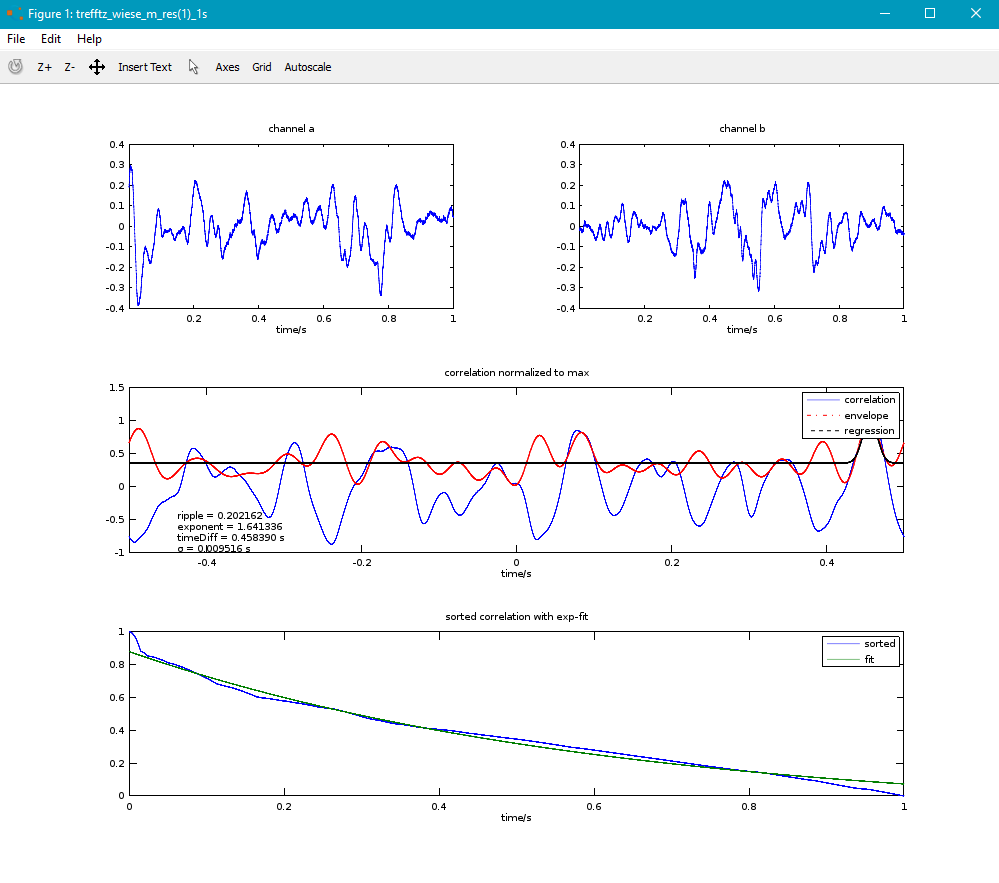
\includegraphics[scale=0.64]{img/trefftz_wiese_m}
\caption{Signal 1}
\label{figure2}
\end{figure}
\paragraph{Beschreibung der KKF} Die Kreuzkorrelationsfunktion schwankt sehr stark über den gesamtem Zeitbereich. Deswegen ist auch die Hüllkurve stark schwankend. Da die Regression über die Hüllkurve berechnet wird, wird diese dem Signal auch nicht gerecht.
\paragraph{Auswertung der Maßzahlen}

\subsubsection{Signal 2 $-$ trefftz$\_$fahrstuhl$\_$m}
\paragraph{Aufnahemsituation} Diese Aufnahme fand im Fahrstuhl des Trefftzbaus statt. Das heißt, der Raum war relativ klein und ist mit schallharten Begrenzungen versehen. Um ein Signal zu erhalten wurde eine Primärschallquelle in Form eines hochwertigen Lautsprechers genutzt.
\paragraph{Signalbeschreibung}
In Abbildung 3 erkennt man sehr gut, dass sich beide Kanäle sehr schnell ändern und einen ähnlichen Verlauf haben. Lediglich die Stärke des Signals ist unterschiedliche. Das stört jedoch nicht für die Berechnung der Maßzahlen. 
\begin{figure}[ht!]
\centering
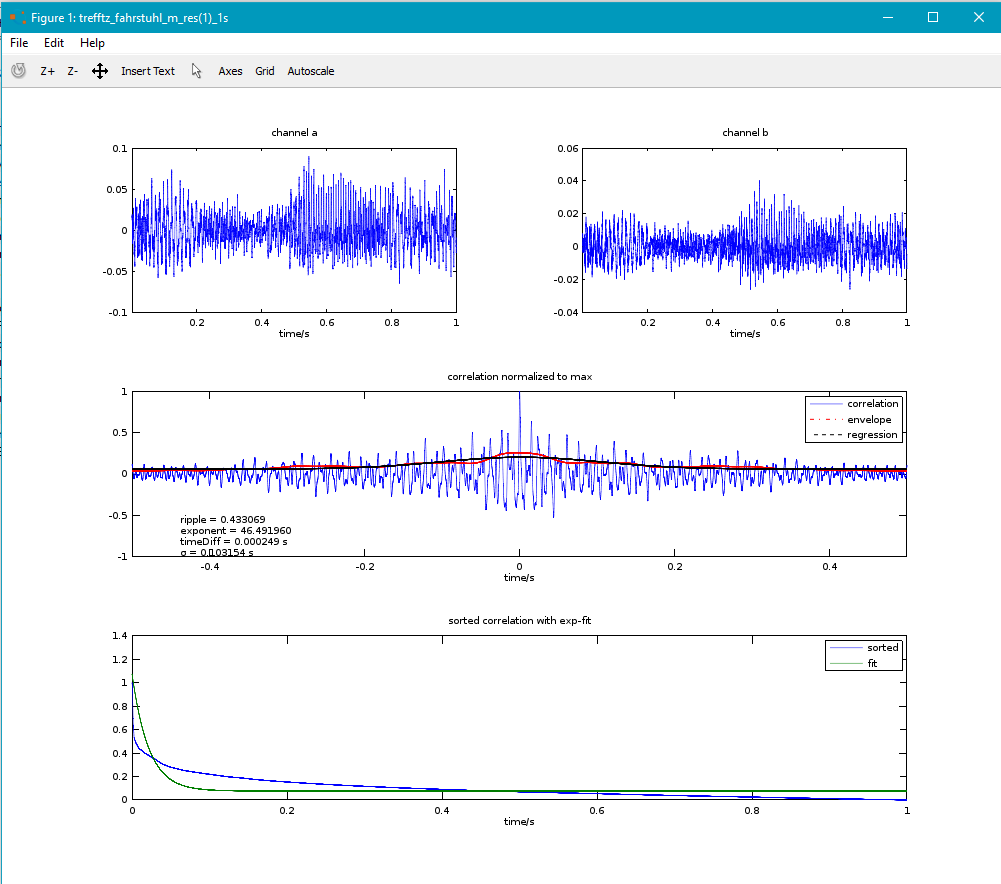
\includegraphics[scale=0.64]{img/trefftz_fahrstuhl_m}
\caption{Signal 2}
\label{figure3}
\end{figure}
\paragraph{Beschreibung der KKF}
Für dieses Signal ist auch an der Kreuzkorrelationsfunktion klar zu sehen, dass es ein Maximum in der Mitte gibt. Das heißt, die Signale sind sich sehr ähnlich. Zu den Seiten nimmt die KKF langsam ab. Für solch einen Verlauf ist die Aussage der Hüllkurve und der Regression sehr gut, da dieses Kreuzkorrelation gut mit einer Gauß-Kurve approxmiert werden kann.
\paragraph{Auswertung der Maßzahlen}

\subsection{Probleme bei der Signalauswahl}
Bei der Signalauswahl ergab sich das Problem, dass man möglichst viele verschiedene Raumsituationen erfassen musste, um möglichst viele verschiedene Daten zu bekommen. Dabei war es jedoch nur schwer möglich vor Ort zu entscheiden, ob die entsprechende Aufnahme sinnvolle Ergebnisse liefert.
In den meisten Situationen war der Lautstärkepegel im Raum zu gering um 20s aufzunehmen, ohne das der Großteil der Aufnahme einfach Rauschen war. Aus diesem Grund haben wir ein zusätzliches Signal erzeugt. Dadurch gibt es jedoch in den meisten Aufnahmen eine Primärquelle, die das Spektrum 

\subsection{Fazit}
